%%%%%%%%%%%%%%%%%%%%%%%%%%%%%%%%%%%%%%%%%%%%%%%%%%%%%%%%%%%%%%%%%%%%%%%%%%%%%%
\subsection{DAQ}
Top view of the DAQ configuration hierarchy is shown in Figure~\ref{figure:daq_config}.

{ \scriptsize
\begin{verbatim}
[local:test_025:S]DAQ>ls -l  
Key name                        Type    #Val  Size  Last Opn Mode Value
---------------------------------------------------------------------------
CFO                             DIR
Subsystems                      DIR
Nodes                           DIR
Tfm                             DIR
# --- artdaq parameters ----    STRING  1     65    12m  0  RWD   ------ first_port = BasePortNumber+PartitionID*PortsPerPartition
PartitionID                     INT32   1     4     12m  0  RWD   11
PortsPerPartition               INT32   1     4     12m  0  RWD   1000
BasePortNumber                  INT32   1     4     12m  0  RWD   10000
#1 ----------------------       STRING  1     64    12m  0  RWD   LocalSubnet and PublicSubnet are used to resolve the host names
PrivateSubnet                   STRING  1     32    12m  0  RWD   131.225.38
PublicSubnet                    STRING  1     32    12m  0  RWD    131.225.38
MIDAS_SERVER_HOST               STRING  1     32    12m  0  RWD   mu2edaq09
# ---- assumption:              STRING  1     67    12m  0  RWD   OnSpill, RocReadoutMode, and EventMode are the same for all DTCs
OnSpill                         INT32   1     4     12m  0  RWD   1
RocReadoutMode                  INT32   1     4     12m  0  RWD   1
EventMode                       INT32   1     4     12m  0  RWD   1
SkipDtcInit                     INT32   1     4     12m  0  RWD   0
# --------------------- 0       STRING  1     42    12m  0  RWD   -------------------- configurable element
MonitoringFrontend              DIR
Enabled                         INT32   1     4     12m  0  RWD   1
Status                          INT32   1     4     12m  0  RWD   0
\end{verbatim}

}

\begin{itemize}
\item
  {\bf CFO} : subdirectory, contains the CFO (Central FanOut module) parameters.
  In the running configuraton there could be only one CFO.
  The CFO parameters are described in subsection \ref{section:cfo}
\item
  {\bf Subsystems} : subdirectory, describes ARTDAQ subsystems
\item
  {\bf Nodes} : subdirectory, describes configurations of the individual trigger farm nodes
\item
  {\bf Tfm} : subdirectory, describes the configuration of the Trigger Farm Manager(TFM)
\end{itemize}


\begin{figure}[H]
  \begin{tikzpicture}
    \node[anchor=south west,inner sep=0] at (0,0.) {
      % \node[shift={(0 cm,0.cm)},inner sep=0,rotate={90}] at (0,0) {}
      \makebox[\textwidth][c] {
        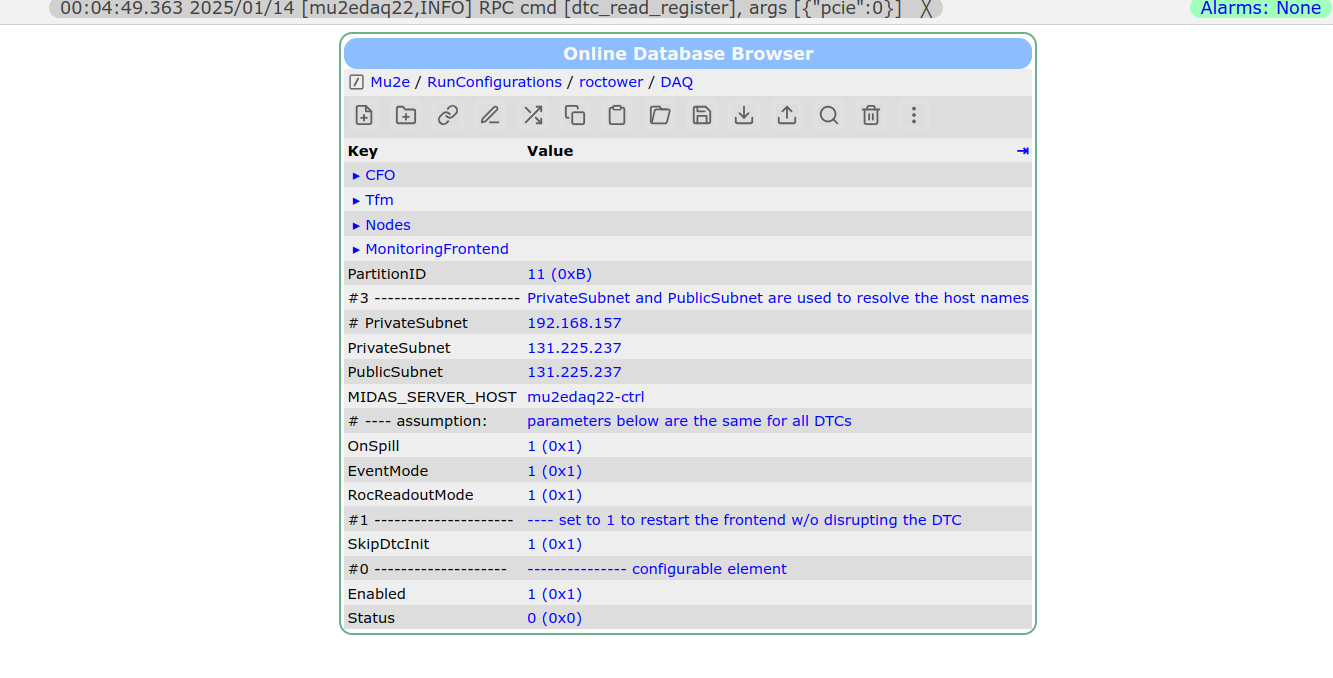
\includegraphics[width=0.95\textwidth]{png/daq_configuration}
      }
    };
    % \node [text width=8cm, scale=1.0] at (14.5,0.5) {$\mu_B$, expected background mean};
    % \node [text width=8cm, scale=1.0, rotate={90}] at (1.5,7.5) { $S_{D}$, ``discovery'' signal strength  };
  \end{tikzpicture}
  \caption{
    \label{figure:daq_config}
    Top level of the DAQ configuration
  }
\end{figure}

It includes configuration of the CFO, the Trigger Farm Manager (TRM), configuration
of the trigger farm nodes and a number of global DAQ parameters.


%%%%%%%%%%%%%%%%%%%%%%%%%%%%%%%%%%%%%%%%%%%%%%%%%%%%%%%%%%%%%%%%%%%%%%%%%%%%%%
\newpage
\subsubsection{CFO configuration}
\label{section:cfo}

Emulated CFO is controlled by the ``emulated CFO frontend''.
That is a frontend with the CFO described a s MIDAS ``periodic equipment''.
When the frontend's periodic readout function is called, a new train of EWMs
is sent to the DTCs.

An example of the emulated CFO configuration is shown in Figure~\ref{figure:cfo_config}.
It includes a link to the configuration of the corresponding FPGA (DTC) 
defined within the same configuration, and a list of the CFO-specific parameters.

\begin{figure}[H]
{ \scriptsize
\begin{verbatim}
[local:test_025:S]CFO>ls -l  
Key name                        Type    #Val  Size  Last Opn Mode Value
---------------------------------------------------------------------------
EmulatedMode                    INT32   1     4     19m  0  RWD   1
Host                            STRING  1     32    19m  0  RWD   mu2edaq09.fnal.gov
NEventsPerTrain                 INT32   1     4     19m  0  RWD   200
EventWindowSize                 INT32   1     4     19m  0  RWD   100
SleepTimeMs                     INT32   1     4     19m  0  RWD   250
DTC -> /Mu2e/RunConfigurations/train_station/DAQ/Nodes/mu2edaq09/DTC0
                                KEY     1     12    >99d 0  RWD   <subdirectory>
Enabled                         INT32   1     4     19m  0  RWD   1
Status                          INT32   1     4     19m  0  RWD   0
\end{verbatim}
}
\caption{
  \label{figure:cfo_config}
  CFO configuration
}
\end{figure}

\begin{itemize}
\item
  {\bf EmulatedMode} : 1: CFO is emulated by a DTC 
  0: external CFO (a separate FPGA)
\item
  {\bf NEventsPerTrain} : number of non-null EWMs in the train
\item
  {\bf EventWindowSize} : event window in units of 25 ns
\item
  {\bf SleepTimeMs}     : the CFO frontend operates as follows: it generates a train of (HB+EWM)'s
  which ends with a null heartbeat, then sleeps for {\bf SleepTimeMs} milliseconds, after which
  the cycle is repeated
\item
  {\bf DTC}     : a link to the corresponding DTC configuration(HB+EWM)'s
\item
  {\bf Enabled} and {\bf Status} : general fields of a configuration element
\end{itemize}

%%%%%%%%%%%%%%%%%%%%%%%%%%%%%%%%%%%%%%%%%%%%%%%%%%%%%%%%%%%%%%%%%%%%%%%%%%%%%%
\subsection {DTC configuration}

\begin{figure}[H]
{ \scriptsize
\begin{verbatim}
[local:test_025:S]mu2edaq09>ls -l DTC0
Key name                        Type    #Val  Size  Last Opn Mode Value
---------------------------------------------------------------------------
Link0                           DIR
Link1                           DIR
Link2                           DIR
Link3                           DIR
Link4                           DIR
Link5                           DIR
PcieAddress                     INT32   1     4     47h  0   RWD  0
EmulatesCFO                     INT32   1     4     2h   0   RWD  1
LinkMask                        UINT32  1     4     3h   0   RWD  1114385
JAMode                          INT32   1     4     2h   0   RWD  1
SampleEdgeMode                  INT32   1     4     2h   0   RWD  0
AutogenDRP                      INT32   1     4     47h  0   RWD  1
EnableClockMarkers              INT32   1     4     2h   0   RWD  0
EnableCFOLinkRX                 INT32   1     4     2h   0   RWD  1
DtcID                           INT32   1     4     47h  0   RWD  18
MacAddrByte                     INT32   1     4     47h  0   RWD  0
# comment_#_2 -------------     STRING  1     54    47h  0   RWD  ------------ tracker-specific 
Station                         INT32   1     4     47h  0   RWD  0
Plane                           INT32   1     4     47h  0   RWD  0
# comment_#_3 -------------     STRING  1     55    47h  0   RWD  --------- configurable element 
Enabled                         INT32   1     4     46h  0   RWD  1
Status                          INT32   1     4     47h  0   RWD  0
\end{verbatim}
  }
\caption{
  \label{figure:dtc_config}
  DTC configuration
}
\end{figure}


%%%%%%%%%%%%%%%%%%%%%%%%%%%%%%%%%%%%%%%%%%%%%%%%%%%%%%%%%%%%%%%%%%%%%%%%%%%%%%
\subsection {ROC configuration}

\begin{figure}[H]
{ \scriptsize
\begin{verbatim}
local:test_025:S]mu2edaq09>ls -l DTC0/Link0
Key name                        Type    #Val  Size  Last Opn Mode Value
---------------------------------------------------------------------------
DetectorElement -> /Mu2e/RunConfigurations/train_station/Tracker/Station_00/Plane_00/Panel_00
#--- configuration element      STRING  1     55    17h  0   RWD  ----------------------------
Enabled                         INT32   1     4     17h  0   RWD  1
Status                          INT32   1     4     17h  0   RWD  0
# -------- subsystem-specific   STRING  1     32    17h  0   RWD  --------- tracker ROC ------
RocDesignInfo                   STRING  1     67    46m  0   RWD  '000000000000000000000000000000000000000000000000000000434f52c7ef'
RocDeviceSerial                 STRING  1     35    46m  0   RWD  'dbf467da6e6387635683a91b34e60abf'
RocGitCommit                    STRING  1     14    46m  0   RWD  READ_DISABLED
\end{verbatim}
}
\caption{
  \label{figure:roc_config}
  ROC configuration
}
\end{figure}

\begin{itemize}
\item
  {\bf DetectorElement} : link to the detector element read out by this ROC.
  The detector element definition is subsystem-specific:
  \begin{itemize}
  \item
    tracker: a single panel
  \item
    calorimeter: 
  \item
    CRV: 
  \item
    STM:
  \item
    EXM: 
  \end{itemize}
\item
  {\bf Enabled, Status} : parameters of the configuration element
\item
  the rest parameters are subsystem-specific. For example, for the tracker they currently include ROC ID (device serial number),
  ROC design info - a label identifying the firmware build, and a git commit of the ROC firmware on github. 
\end{itemize}

%%%%%%%%%%%%%%%%%%%%%%%%%%%%%%%%%%%%%%%%%%%%%%%%%%%%%%%%%%%%%%%%%%%%%%%%%%%%%%
\subsection {Detector element configuration}

\begin{figure}[H]
{ \scriptsize
\begin{verbatim}
[local:test_025:S]Panel_00>ls -l
Key name                        Type    #Val  Size  Last Opn Mode Value
---------------------------------------------------------------------------
Name                            STRING  1     32    17h  0   RWD  MN016
# ------------- #1              STRING  1     55    47h  0   RWD  --------- configurable element ----
Enabled                         INT32   1     4     47h  0   RWD  1
Status                          INT32   1     4     47h  0   RWD  0
# ------------- #2              STRING  1     55    47h  0   RWD  --------- subsystem-specific ----
ID                              STRING  1     32    47h  0   RWD  1
\end{verbatim}
}
\caption{
  \label{figure:detector_element_config}
  Detector element configuration
}
\end{figure}

\begin{itemize}
\item
  {\bf Name}: name of the detector element, required
\item 
  {\bf Enabled, Status} : parameters of the configuration element
\item
  the rest parameters are subsystem-specific and will be added as needed, {\bf ID} is just an example
\end{itemize}

%%%%%%%%%%%%%%%%%%%%%%%%%%%%%%%%%%%%%%%%%%%%%%%%%%%%%%%%%%%%%%%%%%%%%%%%%%%%%%
\subsection{Global configuration frontend}
\label{sec:conf_frontends}

The configuration frontend, as it follows from its name, together with the
Sequencer, manages the hardware configuration at begin run.
It also registers the run transitions in the online run conditions database.


%%%%%%%%%%%%%%%%%%%%%%%%%%%%%%%%%%%%%%%%%%%%%%%%%%%%%%%%%%%%%%%%%%%%%%%%%%%%%% 
\subsection{Node frontends}
\label{sec:node_frontends}

\begin{itemize}
\item
  one monitoring/control frontend per DAQ server. Monitoring:
  \begin{itemize}
  \item
    2 DTC's with 6 ROCs per DTC
  \item
    ARTDAQ processes:
    \begin{itemize}
    \item
      2 boardreaders, N event builders, potentially a data logger, and a dispatcher
    \end{itemize}
  \item
    overall health: amount of free space available
  \end{itemize}
\item
  emulated CFO:
  \begin{itemize}
  \item
    currently : a separate frontend 
  \item 
    make the CFO frontend a separate thread of the node frontend
  \end{itemize}
\item
  external CFO frontend 
\item
  global control frontend:
\end{itemize}

%%%%%%%%%%%%%%%%%%%%%%%%%%%%%%%%%%%%%%%%%%%%%%%%%%%%%%%%%%%%%%%%%%%%%%%%%%%%%%
\subsection{ARTDAQ configuration}

ARTDAQ configuration is stored in ODB. It consists of two parts:
\begin{itemize}
\item
  Trigger Farm Manager (TFM) configuration
\item
  configuration of ARTDAQ subsystems
\item
  configuration of the artdaq processes on each farm node
\end{itemize}

A configuration of a single node is shown in Figure ~\ref{figure:artdaq_configuration}.

\begin{figure}[H]
  \begin{tikzpicture}
    \node[anchor=south west,inner sep=0] at (0,0.) {
      % \node[shift={(0 cm,0.cm)},inner sep=0,rotate={90}] at (0,0) {}
      \makebox[\textwidth][c] {
        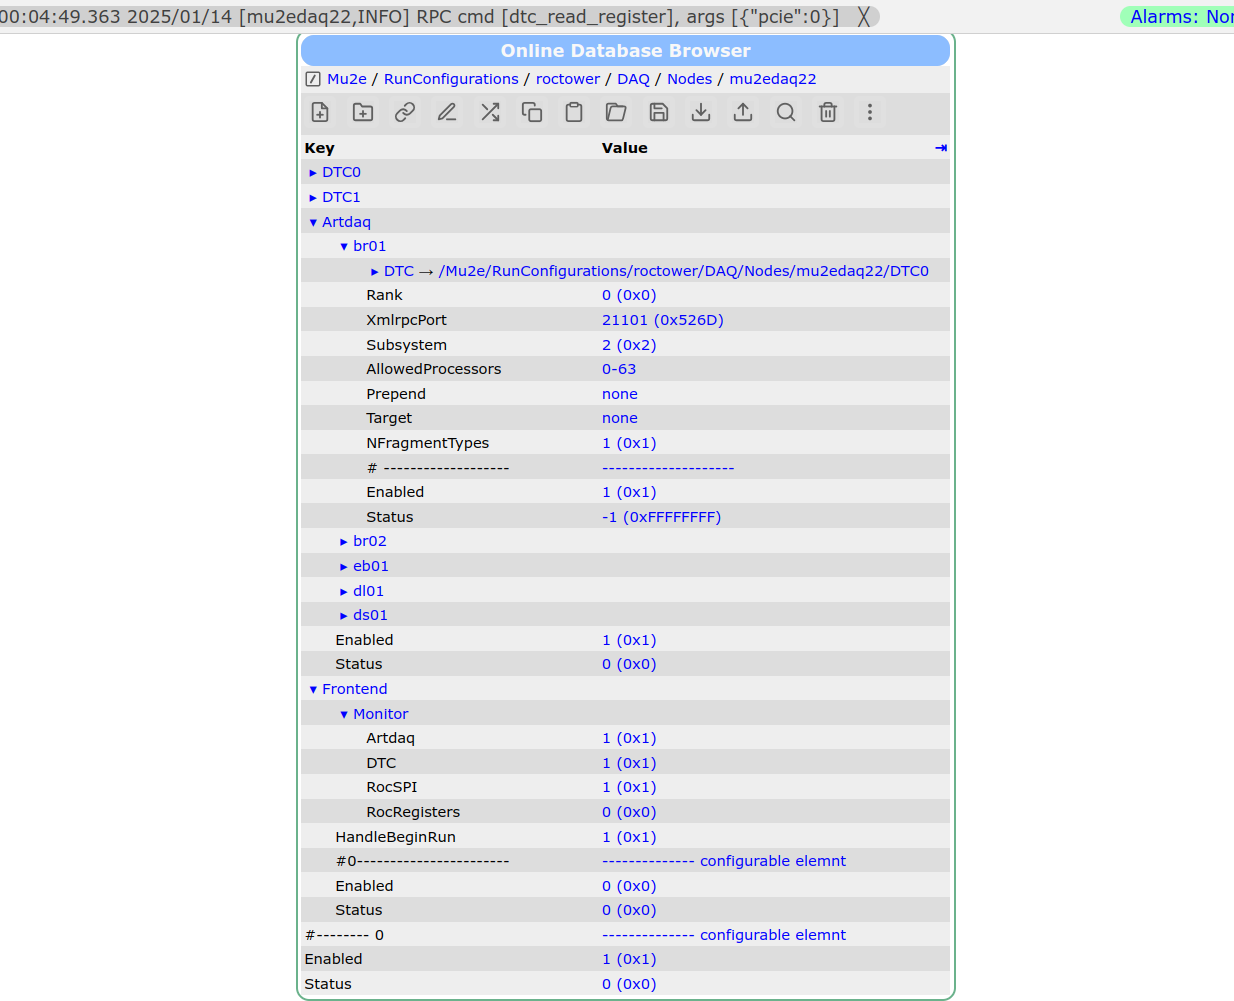
\includegraphics[width=0.95\textwidth]{png/artdaq_configuration}
      }
    };
    % \node [text width=8cm, scale=1.0] at (14.5,0.5) {$\mu_B$, expected background mean};
    % \node [text width=8cm, scale=1.0, rotate={90}] at (1.5,7.5) { $S_{D}$, ``discovery'' signal strength  };
  \end{tikzpicture}
  \caption{
    \label{figure:artdaq_configuration}
    CFO configuration
  }
\end{figure}

It has
\begin{itemize}
\item
  parameters of the DTCs. There could be zero, one, or two DTCs on a farm node.
\item
  parameters of the artdaq processes running on that node.
  Configuration of the ARTDAQ boardreaders has links to the definitions
  of the DTCs they are reading. A boardreader need to know the PCIE address of the DTC
  it is interacting with. At start time, the boardreaders query that information
  from the ODB.
  
\item
  parameters of the node control frontend, including the configuration of the
  slow controls ("Frontend/Monitor")
\end{itemize}

%%%%%%%%%%%%%%%%%%%%%%%%%%%%%%%%%%%%%%%%%%%%%%%%%%%%%%%%%%%%%%%%%%%%%%%%%%%%%%
\subsection{DAQ-to-subdetectors interface}
The DAQ elements are "mapped" linked to the corresponding subdetector elements using ODB links,
as shown in Figure ~\ref{figure:daq_to_tracker_interface}.
\begin{figure}[H]
  \begin{tikzpicture}
    \node[anchor=south west,inner sep=0] at (0,0.) {
      % \node[shift={(0 cm,0.cm)},inner sep=0,rotate={90}] at (0,0) {}
      \makebox[\textwidth][c] {
        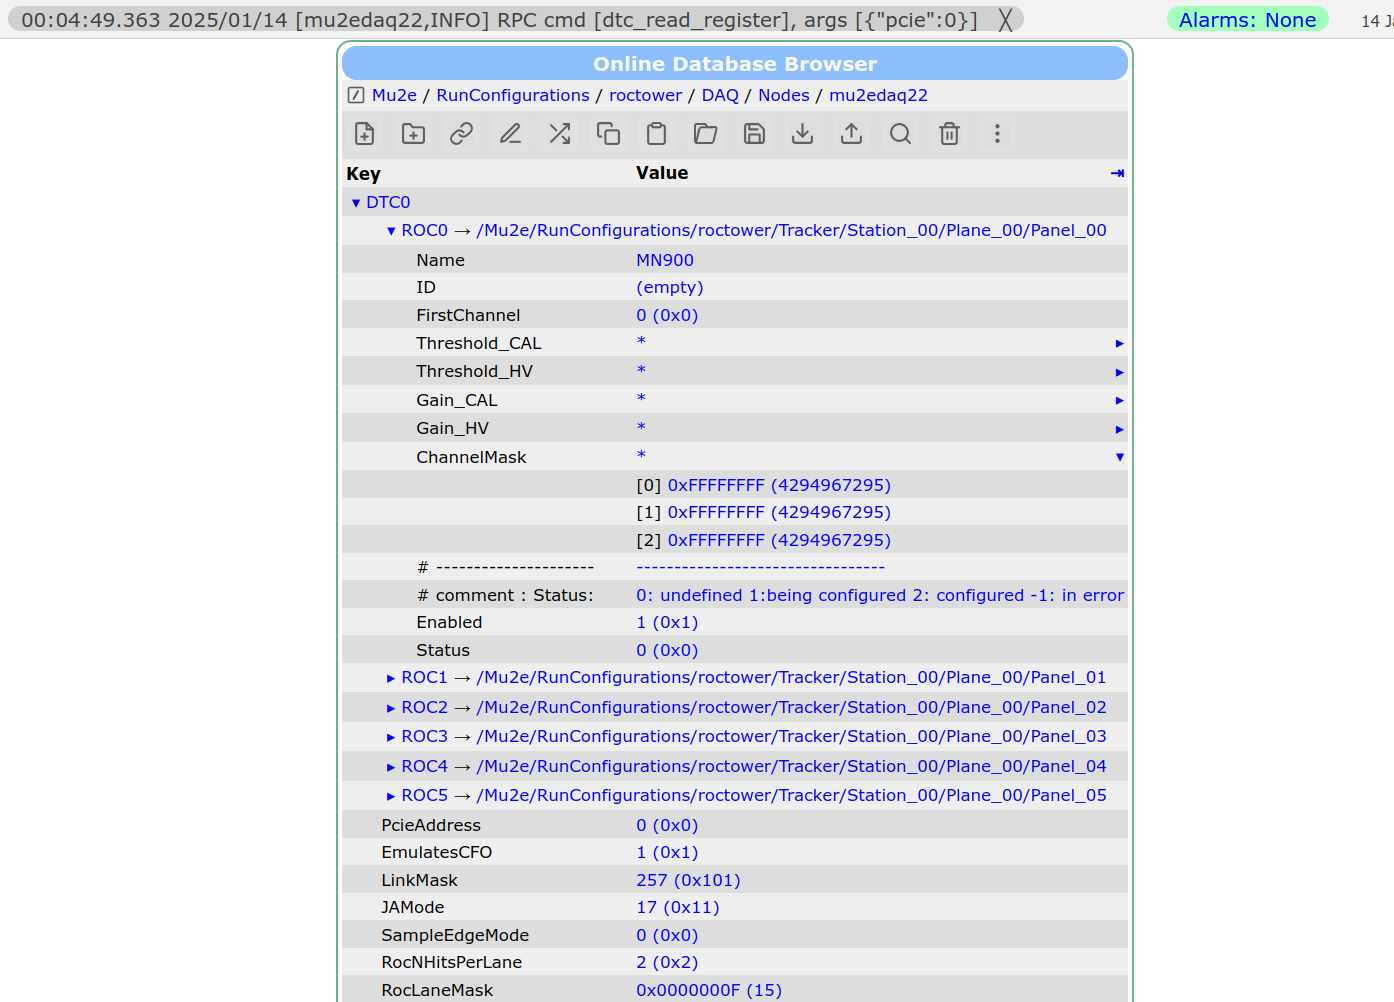
\includegraphics[width=0.95\textwidth]{png/daq_to_tracker_interface}
      }
    };
    % \node [text width=8cm, scale=1.0] at (14.5,0.5) {$\mu_B$, expected background mean};
    % \node [text width=8cm, scale=1.0, rotate={90}] at (1.5,7.5) { $S_{D}$, ``discovery'' signal strength  };
  \end{tikzpicture}
  \caption{
    \label{figure:daq_to_tracker_interface}
    CFO configuration
  }
\end{figure}

A DAQ node has links to the DTCs installed on that node, and the tracker DTC ROCs shown have
links to the definitions of the tracker panels they are reading.

%%% Local Variables:
%%% mode: latex
%%% TeX-master: t
%%% End:
